\documentclass{emulateapj}
\submitted{{\it Submitted for publication in ApJ}}
\usepackage{multirow,color,wrapfig,ulem}
\usepackage {graphicx}
\usepackage{graphics}
\usepackage[dvips]{epsfig}

%=========================================================================
%		INTERNAL MACROS
%=========================================================================
\def\be{\begin{equation}}
\def\ee{\end{equation}}
\def\ba{\begin{eqnarray}}
\def\ea{\end{eqnarray}}

% To highlight comments 
\definecolor{red}{rgb}{1,0.0,0.0}
\newcommand{\red}{\color{red}}
\definecolor{darkgreen}{rgb}{0.0,0.5,0.0}
\newcommand{\SRK}[1]{\textcolor{darkgreen}{\bf SRK: \textit{#1}}}
\newcommand{\SRKED}[1]{\textcolor{darkgreen}{\bf #1}}
\newcommand{\before}[1]{\textcolor{red}{ #1}}
\newcommand{\after}[1]{\textcolor{darkgreen}{ #1}}

\newcommand{\LCDM}{$\Lambda$CDM~}
\newcommand{\beq}{\begin{eqnarray}}  
\newcommand{\eeq}{\end{eqnarray}}  
\newcommand{\zz}{$z\sim 3$} 
\newcommand{\avg}[1]{\langle{#1}\rangle}  
\newcommand{\ly}{{\ifmmode{{\rm Ly}\alpha}\else{Ly$\alpha$}\fi}}
\newcommand{\hMpc}{{\ifmmode{h^{-1}{\rm Mpc}}\else{$h^{-1}$Mpc}\fi}}  
\newcommand{\hGpc}{{\ifmmode{h^{-1}{\rm Gpc}}\else{$h^{-1}$Gpc}\fi}}  
\newcommand{\hmpc}{{\ifmmode{h^{-1}{\rm Mpc}}\else{$h^{-1}$Mpc}\fi}}  
\newcommand{\hkpc}{{\ifmmode{h^{-1}{\rm kpc}}\else{$h^{-1}$kpc}\fi}}  
\newcommand{\hMsun}{{\ifmmode{h^{-1}{\rm {M_{\odot}}}}\else{$h^{-1}{\rm{M_{\odot}}}$}\fi}}  
\newcommand{\Mmin}{{\ifmmode{{M_{\rm min}}}\else{${M_{\rm min}}$}\fi}}
\newcommand{\mmin}{{\ifmmode{{M_{\rm min}}}\else{${M_{\rm min}}$}\fi}}
\newcommand{\mmax}{{\ifmmode{{M_{\rm max}}}\else{${M_{\rm max}}$}\fi}}
\newcommand{\lmmin}{{\ifmmode{{\log M_{\rm min}}}\else{${\log M_{\rm min}}$}\fi}}
\newcommand{\lmmax}{{\ifmmode{{\log M_{\rm max}}}\else{${\log M_{\rm max}}$}\fi}}

\newcommand{\Mmax}{{\ifmmode{{M_{\rm max}}}\else{${M_{\rm max}}$}\fi}}
\newcommand{\dm}{{\ifmmode{{\Delta M}}\else{$\Delta M$}\fi}}
\newcommand{\dlm}{{\ifmmode{{\Delta \log M}}\else{$\Delta \log M$}\fi}}
\newcommand{\focc}{{\ifmmode{{f_{\rm occ}}}\else{${f_{\rm occ}}$}\fi}}

\newcommand{\Msun}{{\ifmmode{{\rm {M_{\odot}}}}\else{${\rm{M_{\odot}}}$}\fi}}  
\newcommand{\msun}{{\ifmmode{{\rm {M_{\odot}}}}\else{${\rm{M_{\odot}}}$}\fi}}  
\newcommand{\lya}{{Lyman$\alpha$~}}
\newcommand{\clara}{{\texttt{CLARA}}~}
\newcommand{\rand}{{\ifmmode{{\mathcal{R}}}\else{${\mathcal{R}}$ }\fi}}  
%SAMPLES


%MY COMMANDS #############################################################
\newcommand{\sub}[1]{\mbox{\scriptsize{#1}}}
\newcommand{\dtot}[2]{ \frac{ d #1 }{d #2} }
\newcommand{\dpar}[2]{ \frac{ \partial #1 }{\partial #2} }
\newcommand{\pr}[1]{ \left( #1 \right) }
\newcommand{\corc}[1]{ \left[ #1 \right] }
\newcommand{\lla}[1]{ \left\{ #1 \right\} }
\newcommand{\bds}[1]{\boldsymbol{ #1 }}
\newcommand{\oiint}{\displaystyle\bigcirc\!\!\!\!\!\!\!\!\int\!\!\!\!\!\int}
\newcommand{\mathsize}[2]{\mbox{\fontsize{#1}{#1}\selectfont $#2$}}
\newcommand{\eq}[2]{\begin{equation} \label{eq:#1} #2 \end{equation}}
\newcommand{\lth}{$\lambda_{th}$ }
\newcommand{\reff}{{\ifmmode{r_{\mbox{\tiny eff}}}\else{$r_{\mbox{\tiny eff}}$}\fi}}
%#########################################################################

%TO DO COMMANDS. Highlight region that needs extra work  #############################################################
\newcommand{\todo}{\ifmmode \text{\Huge{\(\bullet\)}} \else {\Huge$\bullet$}\fi}
% \newcommand{\todo}{\ifmmode {\Huge \bullet} \else {\Huge$\bullet$}\fi}
\newcommand{\tido}{\ifmmode {\bullet} \else $\bullet$\fi}
\newcommand{\REFS}{(\todo REFS) }
\newcommand{\toref}{(\todo REFS)}
%#########################################################################



\begin{document}
%=========================================================================
%		FRONT MATTER
%=========================================================================
\title{Satellite Alignments in Galaxy Pairs}
\author{
  Ver\'onica Arias \thanks{v.arias@uniandes.edu.co}$^{1}$,
  Jaime E. Forero-Romero \thanks{je.forero@uniandes.edu.co}$^{2}$ 
}

\affil{
$^1$Departamento de F\'{i}sica, Universidad de los Andes, Cra. 1
No. 18A-10, Edificio Ip, Bogot\'a, Colombia\\
}

\begin{abstract}
Alineaciones.
\end{abstract}

\keywords{
Galaxies: halos --- Galaxies: high-redshift --- Galaxies: statistics
--- Dark Matter --- Methods: numerical 
}

\section{Introduction}

%
%Observational evidence of planes is everywhere (where we can see them). MW, M31, Centaurus A.\\
%
%Not so evident in simulations:\\
%
%Millenium II Baumgardt, Ibata, Pawlowski\\
%
%Clues Gillet está pero diferente\\
%
%Plane claims:\\
%Libeskind: preferential direction for accretion.\\
%Sawala: planes are there when baryonic physics is included.\\
%Buck: planes are easy to form at early times, when DM filaments are very thin. In high redshift galaxies galaxies, planes are everywhere.\\
%
%Other explanations: Kroupa: tidal dwarfs\\
%Fouquet\\
%
%
%
% 
%Following a bit on the claim by Sawala that barionic physics are important when looking for planes, WE look in Illustris and Elvis simulations to try and understand why barionic physics results in planar distribution of satellites.

%\subsection{Evidencias observacionales de planos:}
\noindent Since the early works of (el que libeskind dice que habló de
eso primero) and Lynden-Bell (1976), the observed anisotropic
distribution of satellite galaxies in the Local Group has been a key
point in the discussion of galaxy formation models within $\Lambda$CDM
cosmology. These pioneer papers described that the then known satellite
galaxies of the Milky May (MW) were distributed roughly following the plane
that contained the Magelanic clouds and their stellar tails. This
anisotropic distribution was further studied in the work of Pawlowski
et. al. (2012), where they included all the known MW satellite galaxies (XXX
more than in the original Lynden-Bell paper) as well as some MW globular
clusters, and found that they are all contained in what they call a
"Vast Plane Of Satellites" (VPOS). This structure is around 30kpc thick and
is perpendicular to the stellar disc of the MW galaxy. This plane of
satellites was considered a rarity until the PAndAS survey of the
Andromeda (M31) galaxy and its halo (missing reference on the survey)
provided a complete sample of the satellite galaxy population (above a
XXXX magnitude) of our neighboring galaxy, allowing their consistent distance
estimations (Conn et al. 2012). In a groundbreaking work, Ibata et
al. (2013) found that 15 out of the 30 satellites are in a planar
structure that is 15kpc thick and has an extension of 400kpc.
Additionally, from line of sight velocity measurements, they
found that the structure has an apparent coherent rotation, with the
satellites south of M31 moving away from us and those north of M31
coming towards us. This apparent organized rotation of satellite galaxies was also
statistically found to occur in diametrically opposed 
pairs of satellites from the SDSS (Ibata et al. 2014), although this
results were contested in a follow up paper by Cuatun et al. (2014).  

These discoveries of the planes in M31 and the MW were followed by the
remark from Shaya et al. (2013) that the other satellite galaxies in
M31 could be part of a second plane, further reinforcing the idea that
satellites in the local group are not isotropically distributed.
Despite the challenges in estimating distances to the satellites
galaxies, Tully et al. managed to go beyond the local group and found
two planes of satellites galaxies in Centaurus A, making a clearer
case for the planes of satellites: in all the galaxies where distance
measurements could be performed evidence of satellite planar
structures have been found.\\

These observed planes present a challenge for current galaxy formation
models (Pawlowski et al. 2014)


%The VPOS (Pawlowski et al 2012: https://arxiv.org/abs/1204.5176)\\
%A vast thin plane of corrotating dwarf galaxies orbiting the Andromeda
%Galaxy (Ibata et al 2013)\\
%Corotation in SDSS data (Ibata et al 2014)\\
%There was a reply to this paper (A new spin on disks of satellite
%galaxies, Cuatun et al 2014)\\
    %Planes in Centaurus A (Tully et al 2015)\
%paper con los dos planos MW yM31
%>https://arxiv.org/pdf/1307.6210v1.pdf
\
%Varios papers de pawlowski que muestran que los nuevos sat\'elites de
%MW estan en el plano, que el plano no se debe al Sdss footprint, que
%los globular clusters tambien estan en el plano... etc,\\ 
%Papers de Conn donde encuentra el plano\\

%\subsection{B\'usqueda de planos en simulaciones:}
\noindent A comparison of the distribution of satellite galaxies
around Andromeda and the results of $\Lambda$CDM simulations (Bahl and
Baumgardt 2013) Encuentran planos en Millenium II.\\
A thousand shadows of Andromeda: rotating planes of satellites in the
Millennium-II cosmological simulation (Ibata et al 2013) dicen que el
paper de Bahl y Baumgardt est\'a mal y que no hay planos en millenium
II\\
Co-orbiting satellite galaxy structures are still in conflict with the
distribution of primordial dwarf galaxies (Pawlowski et al 2014)\\
Co-orbiting planes of sub-halos are similarly unlikely around paired
and isolated hosts (Pawlowski et al 2014)\\
Vast planes of satellites in a high resolution simulation of the Local
Group: comparison to Andromeda (Gillet et al 2014). finds a plnes
similar to that of M31 in Clues simulations.\\
Planes of satellite galaxies: when exceptions are the rule (Cautun et
al 2015) encuentra que 10 por ciento de los halos tienen planos
iguales o m\'as prominentes que los del LG.\\

\subsection{Posibles or\'igenes de los planos:}
\noindent Preferential accretion (Libeskind et al 20??)\\
Alignments with the cosmic web (Tempel et al 20??)\\
The vast thin plane of M31 co-rotating dwarfs: an additional fossil
signature of the M31 merger and of its considerable impact in the
whole Local Group (Hammer et al 2013) Major merger in M31-MW system
plane galaxies are tidal dwarfs (n-body simulations)\\
Kroupa tiene todo un carretazo de que las dwarfs son todas tidal
dwarfs\\
MIRAR lo que est\'a haciendo Pierre Alan Duc con tidal dwrafs porque en
una conferencia este a;o habl\'o de un posible escenario
intermedio...\\
Evidence for Early Filamentary Accretion from the Andromeda Galaxy's
Thin Plane of Satellites (Buck et al 2015)\\
Alignments between galaxies, satellite systems and haloes (Cautun et al
2016) NO LO HE LEIDO...

\subsection{Problemas con esas explicaciones:}
The Vast Polar Structure of the Milky Way and Filamentary Accretion of
Sub-Halos (Pawlowski et al 2012)\\
Paper de Collins (2013 y 2016) donde explica que no hay doferencias en
las propiedades de los on-plane y los off-plane satellites\\
Problemas con la estabilidad a largo plazo de los planos: Bowden et al
2012, Gonzales et al 2015...\\
The Plane Truth: Andromeda analog thin Planes of Satellites are not
kinematical coherent structures (Buck et al 2015)\\

 


\section{Illustris simulation}

\section{Sample Selection}

We select all halos with maximum circular velocities in the
range 150 km s$^{-1}$ $<V_{\rm max}<$ 350 km s$^{1}$.
We exclude sub-halos from this selection.
From this set we construct a sample of pairs as follows.
For each halo $A$ we find its closest halo $B$, if halo $A$ is also
the closest to halo $B$, the two halos are considered as a pair. 
Another way to phrase this selection is that pairs do not have
neighbors closer than the pair's distance.
We exclude the pairs that are closer than
There are $53$ pairs with those conditions in the simulation.

We extract from the simulation spheres of $2$ \hMpc in radius around
the pair's center of mass. 
We use this information to exclude all the pairs that have separations
smaller than the sum  of their virial radii, i.e. we exclude
interacting pairs. 
This reduces to $49$ the number of pairs in the sample.

We count the number of galaxies with $M_V<-9$ inside the virial
radius of each halo, including the central galaxy.
We only keep pairs where both halos have 5 bright galaxies at least. 
This reduces the sample to $24$ pairs. 
We call this sample the Full  Sample.

From the Full Sample we build a second sample based on the pairs' kinematics. 
Figure \ref{fig:samples} shows the co-moving separation and relative
speed between the two halos in the pair.
The stars in the Figure represent the pairs with a separation in the
range $0.75\hMpc <R_{AB}< 1.50\hMpc$ and relative velocity in the
range $V_{AB}>100$ km s$^{-1}$, which are close to the Local Group
Observed values.
We call this sample the LG Sample.

The number of pairs in the Full Sample is consistent with previous
calculations. 
\cite{ForeroRomero2013} performed a study of the LG kinematics using a
cosmological N-body simulation as a benchmark. 
In their study, using criteria similar to ours to define the Full
Sample, they found 1923 pairs in a volume of $250^3$ $h^{-3}$
Mpc$^{3}$. 
With the same number density we expect to find $52$ pairs in the
volume of the Illustris simulation, which is very close to the actual
number of $49$ pairs.

In the same study they found 158 pairs with broad kinematic
characteristics, similar to the definition of our LG sample. 
This represents a reduction of a factor of $12$ from their General
Sample. 
With those numbers in mind we would expect to keep at least $4$ pairs
in the Illustris volume. 
Given that our conditions are slightly more relaxed (we do not ask for
isolation criteria from massive halos) we end up with a larger sample
size, but still consistent with the fact that LG-like pairs are
scarce.  

\citep{2011MNRAS.411.1525L} Measure the infall direction of satellites
in a DM only simulation of one pair of LG halos in a constrained
simulation. There is a definite infall direction but it's not
quantified in terms of the cosmic web.
 
\citep{2012MNRAS.424...80P} Compare the kinematic structure of the MW
satellites against DM only simulation of high resolutions halos from
the Via Lactea and Aquarius projects.  Cannot find a similar kinematic
structure (i.e. the orbital poles of the MW satellites) in the
simulations. 

\citep{2014MNRAS.443.1274L} Measure the infall direction of satellites
with respect to the V-web. They do it in a DM cosmological simulation
(64 Mpch, 1024 3 particles). They find that infall is done along the
e3 (i.e. filament) direction.

\citep{2015MNRAS.450.2727T} They measure the angle between satellites
and the direction defined by filaments (Bissous filament finder )to
find a signal both in SDSS and the semi-analytic galaxies in the
Millennium Simulation.  

\citep{2015ApJ...799..212L} Detection of alignment of satellites along
the direction defined by filaments (velocity shear cosmic web) on the
SDSS DR7.



\citep{2016MNRAS.457.1931S} Uses the APOSTLE simulation (12 pairs) to study the
spatial anisotropy the 11 brightest satellites. THe anisotropy is
quantified the reduced inertia tensor. Still the MW is more
anisotropic than all but one of the 24 halos. The analysis is not very
thorough and do not show the resulting distribution. Does not compare
the results of using DM information only. 

\citep{2015ApJ...815...19P} argue that the result from
\citep{2016MNRAS.457.1931S} is a produc of using a metric that ignores
the radial position of the galaxies. They use the ELVIS suite to
compare the two analysis methods: reduced vs. full inertia tensor. 

\citep{2016arXiv160501728S} Use the eagle simulation to study the
alignment of satellites with respect to the central galaxy. They find
a weak alignment. Around $20\%$ of the systems have a misalignment
angle larger than the value observed for the Milky Way. They do not
study DM only simulations and do not narrow down the signal to pairs. 

\citep{2016arXiv160601516L} Using SDSS DR10 studied galaxy pairs. They find
that satellites tend to accumulate towards the companion galaxy. There
are up to $\sim 10\%$ more satellites in the space between the pair
than expected from an uniform distribution



\begin{figure}
\centering
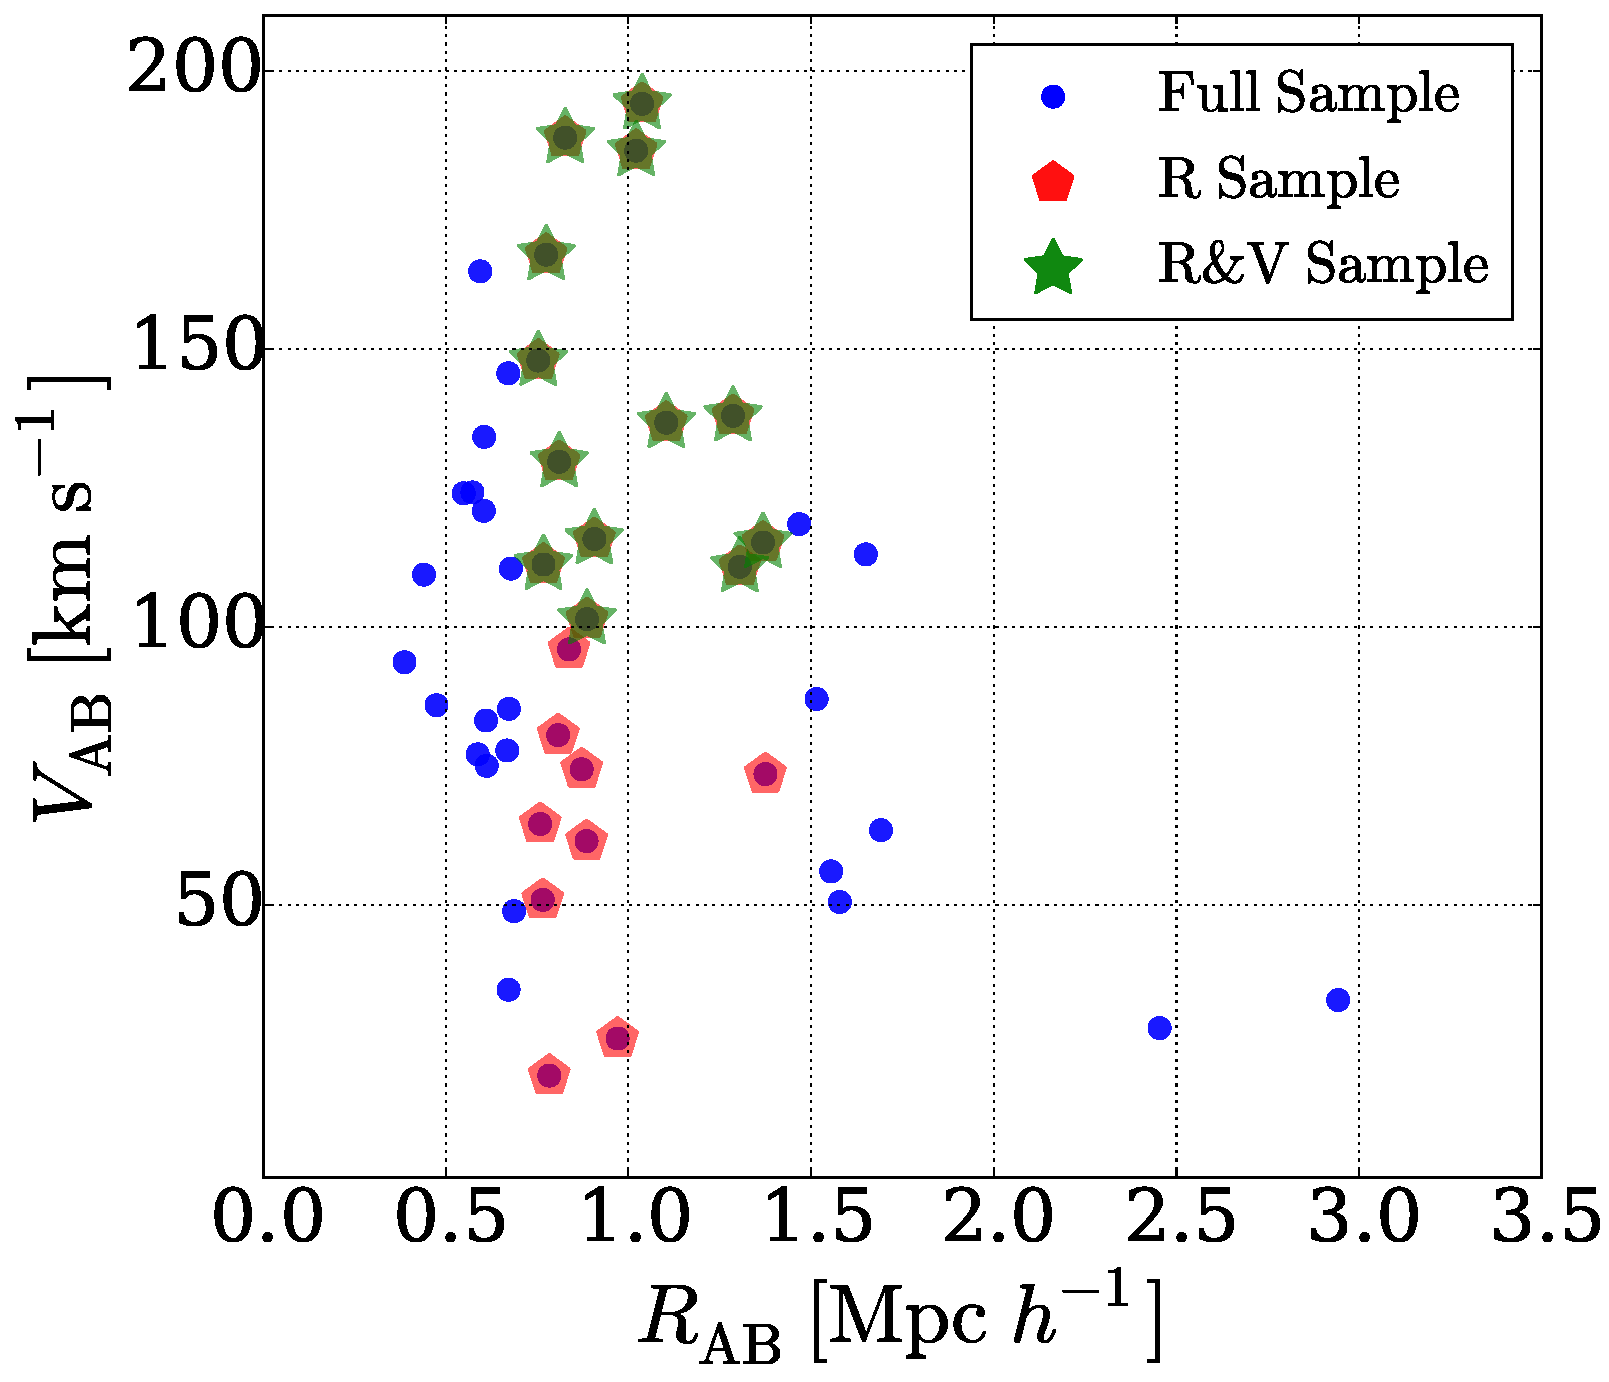
\includegraphics[width=\hsize]{v_r_pairs.pdf}\\
\caption{Halo pair samples used in this paper located in the
  plane of relative comoving velocity $V_{AB}$ versus relative
  distance $R_{AB}$ between the two halos in the pair.
  The R\&V sample is the closest to the separation and kinematic
  conditions observed in the Local Group.} 
\label{fig:samples}
\end{figure}

%\begin{figure}
%\centering
%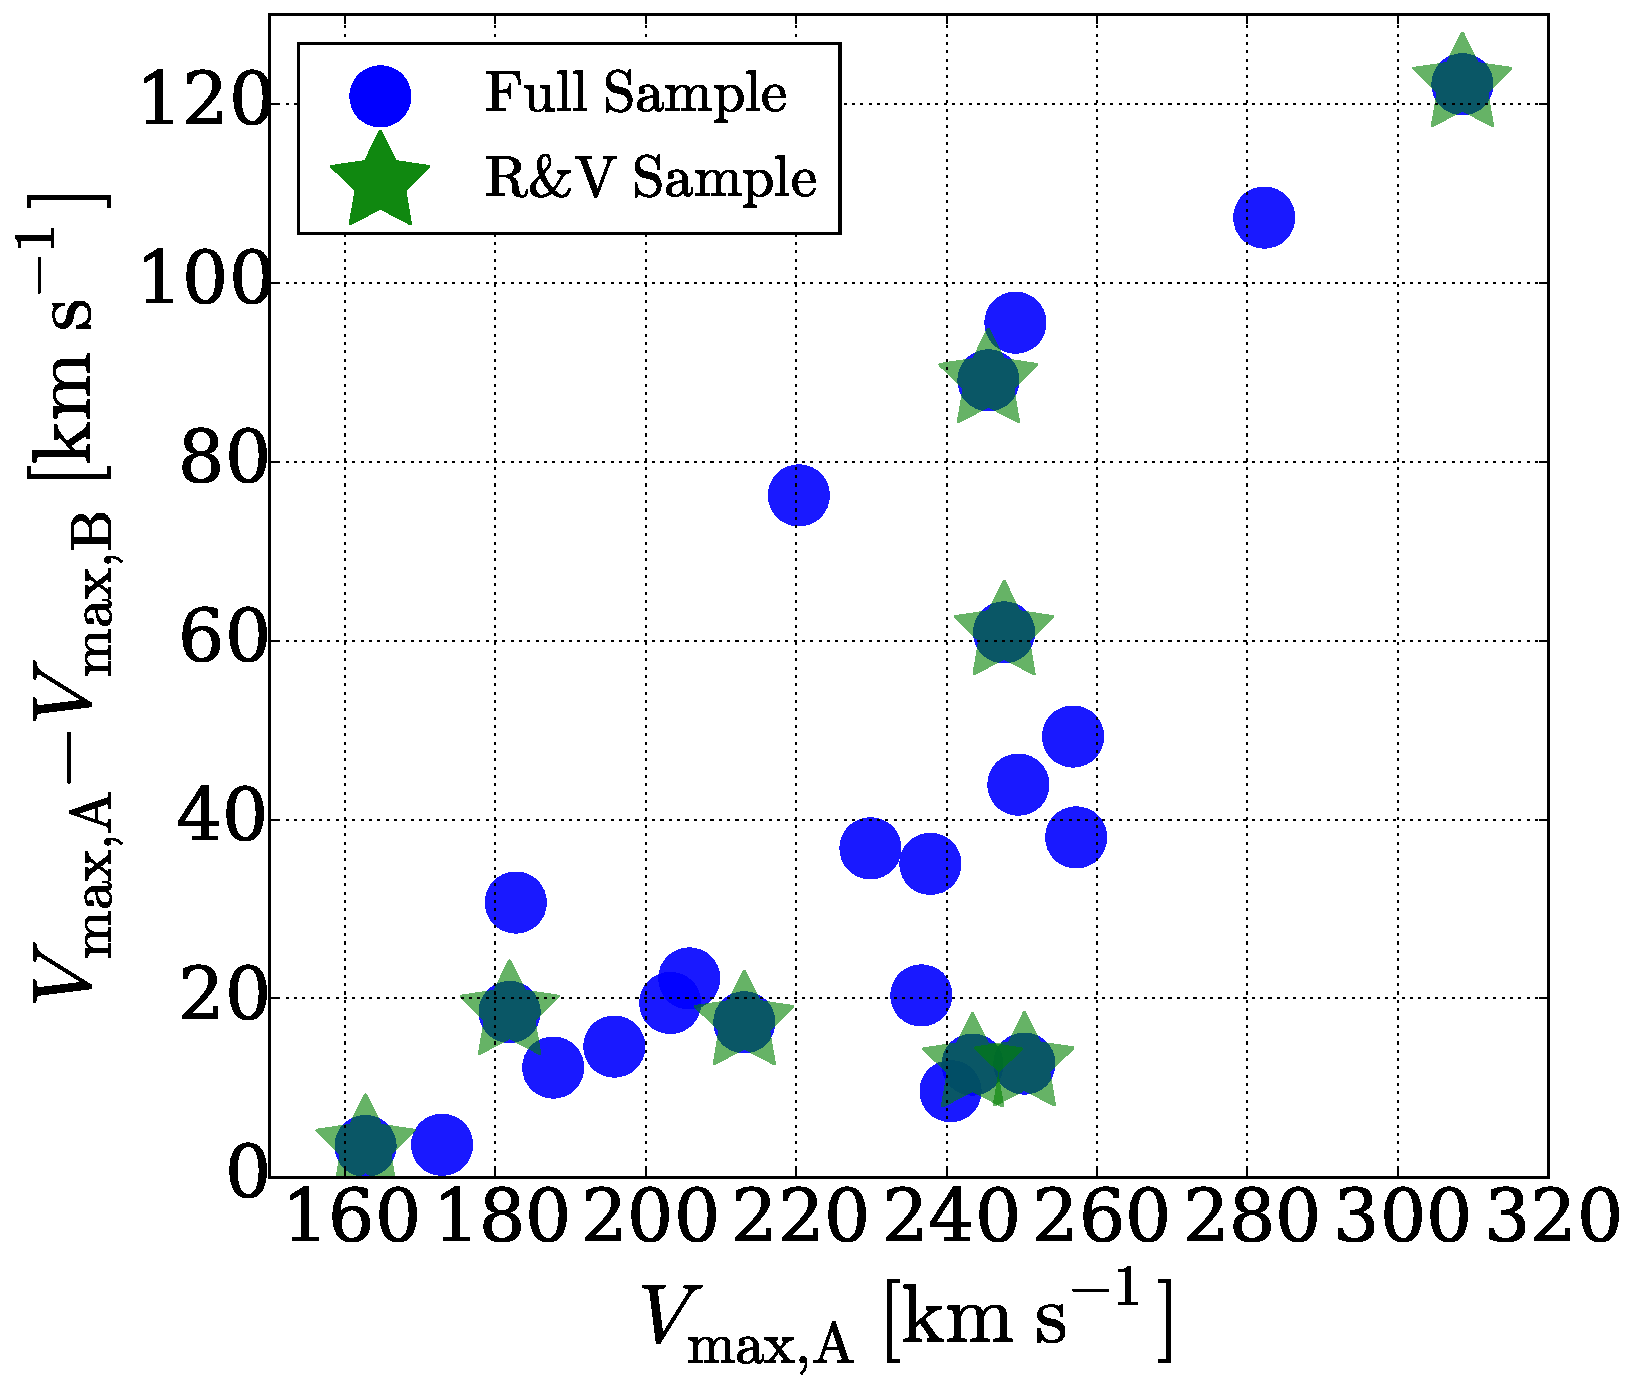
\includegraphics[width=\hsize]{v_circ_pairs.pdf}\\
%\caption{Diference between the maximum circular velocity $V_{max}$ for the two
%  halos in the pair as a function of $V_{max}$ for the massive halo in
%  the pair.}
%\label{fig:vcirc}
%\end{figure}

\begin{figure}
\centering
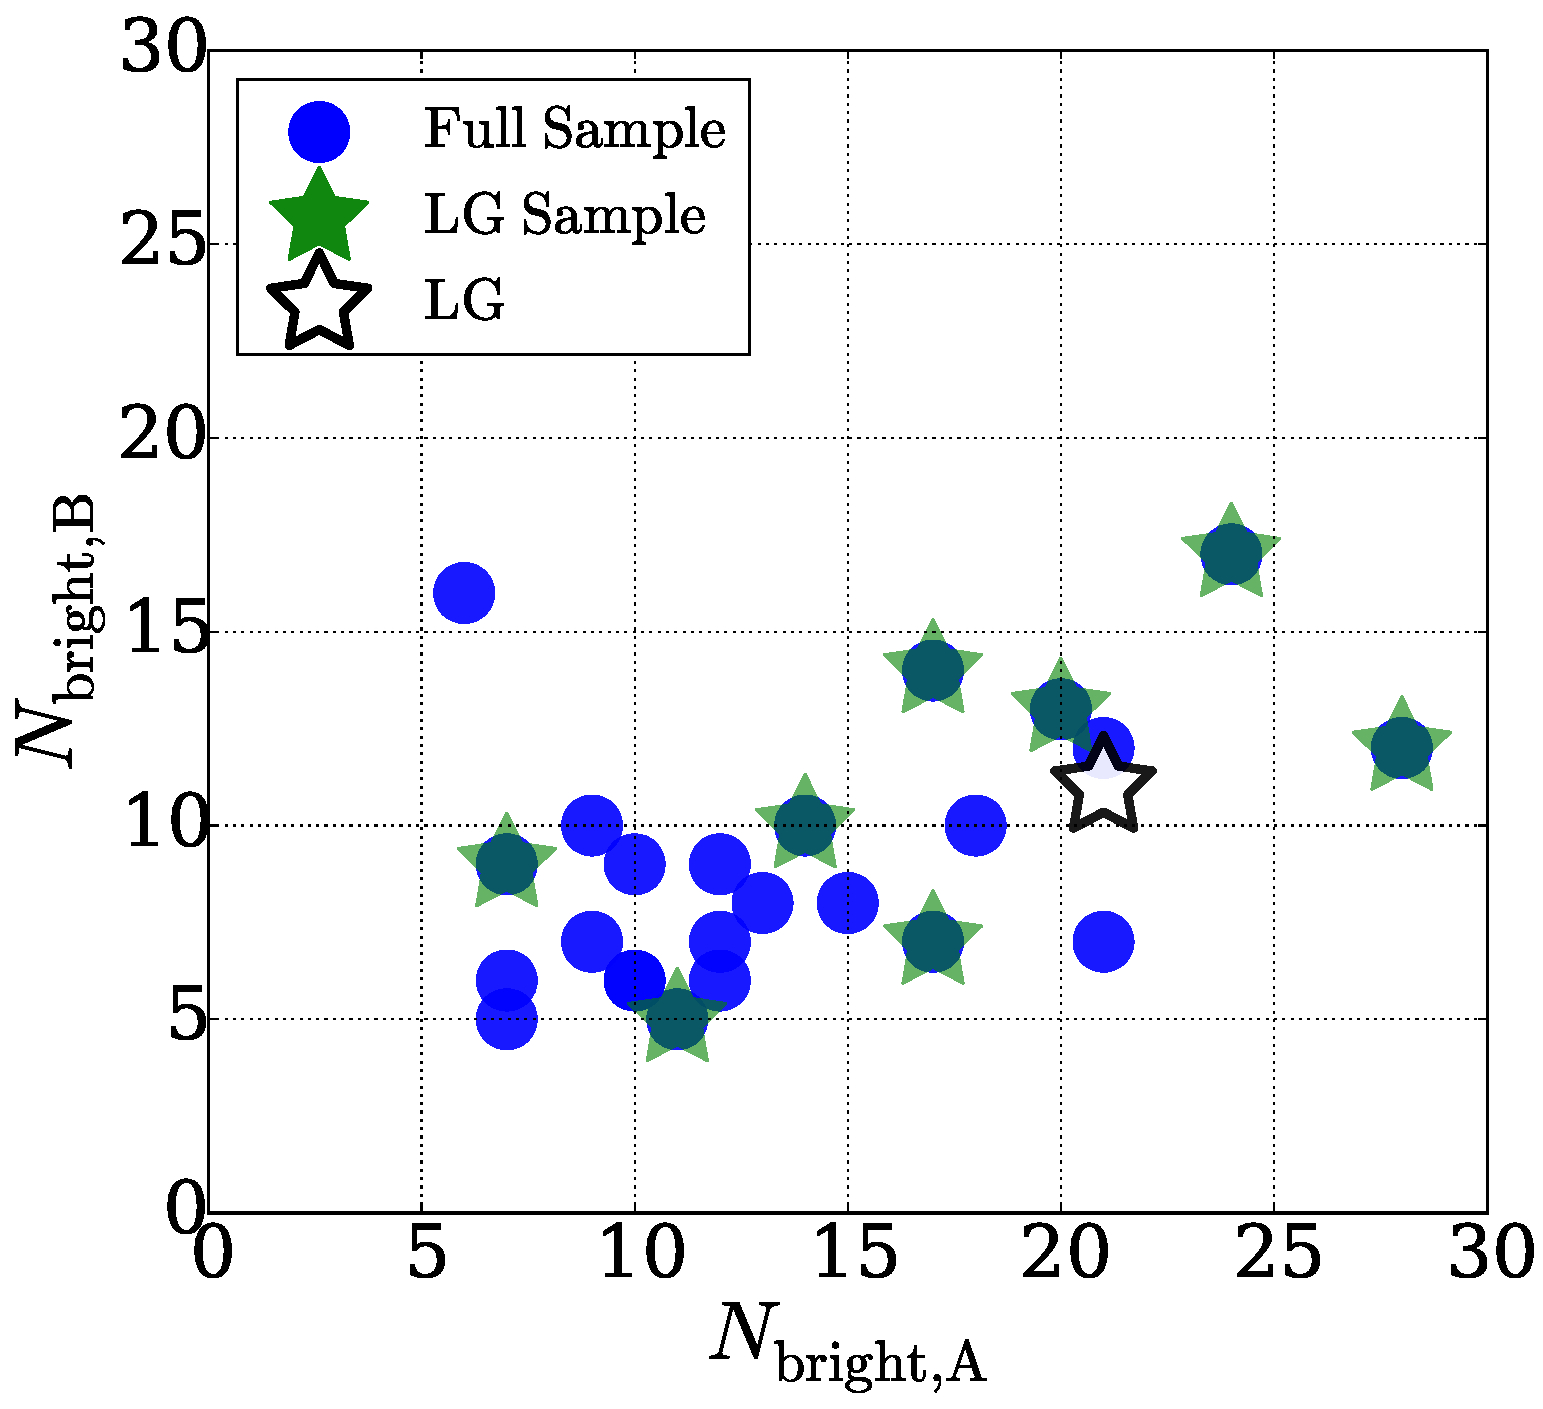
\includegraphics[width=\hsize]{n_structure.pdf}\\
\caption{Number of bright substructures ($M_{B}<-9$) and dark matter
  substructures.}
\label{fig:nstructure}
\end{figure}



\begin{figure}
\centering
\includegraphics[width=\hsize]{axratio_dark_bright.pdf}\\
\caption{Axis ratio of luminous satellites versus the axis ratio for
  dark subhalos.}
\label{fig:StreamPlaneOrbit}
\end{figure}


\begin{figure*}
\centering
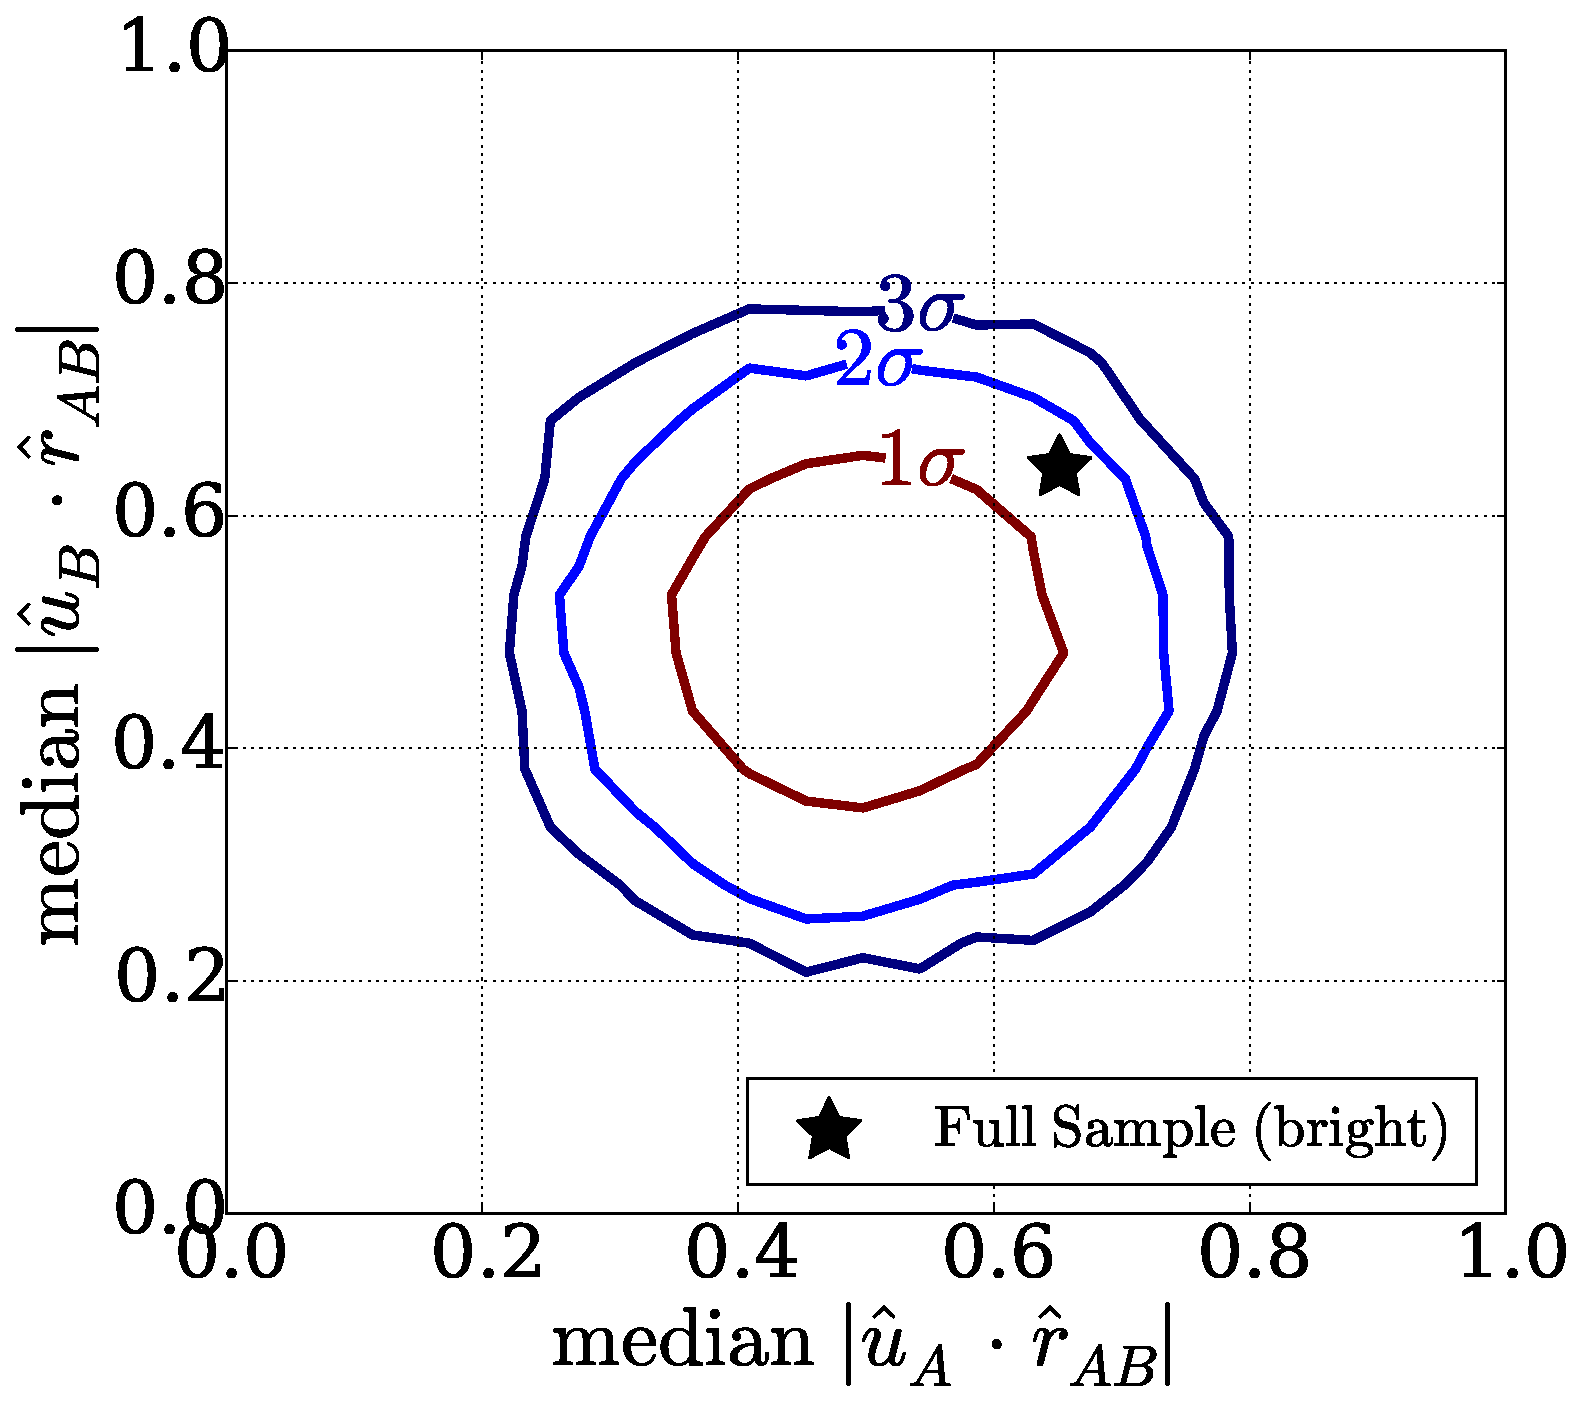
\includegraphics[width=0.48\hsize]{significance_full_bright.pdf}
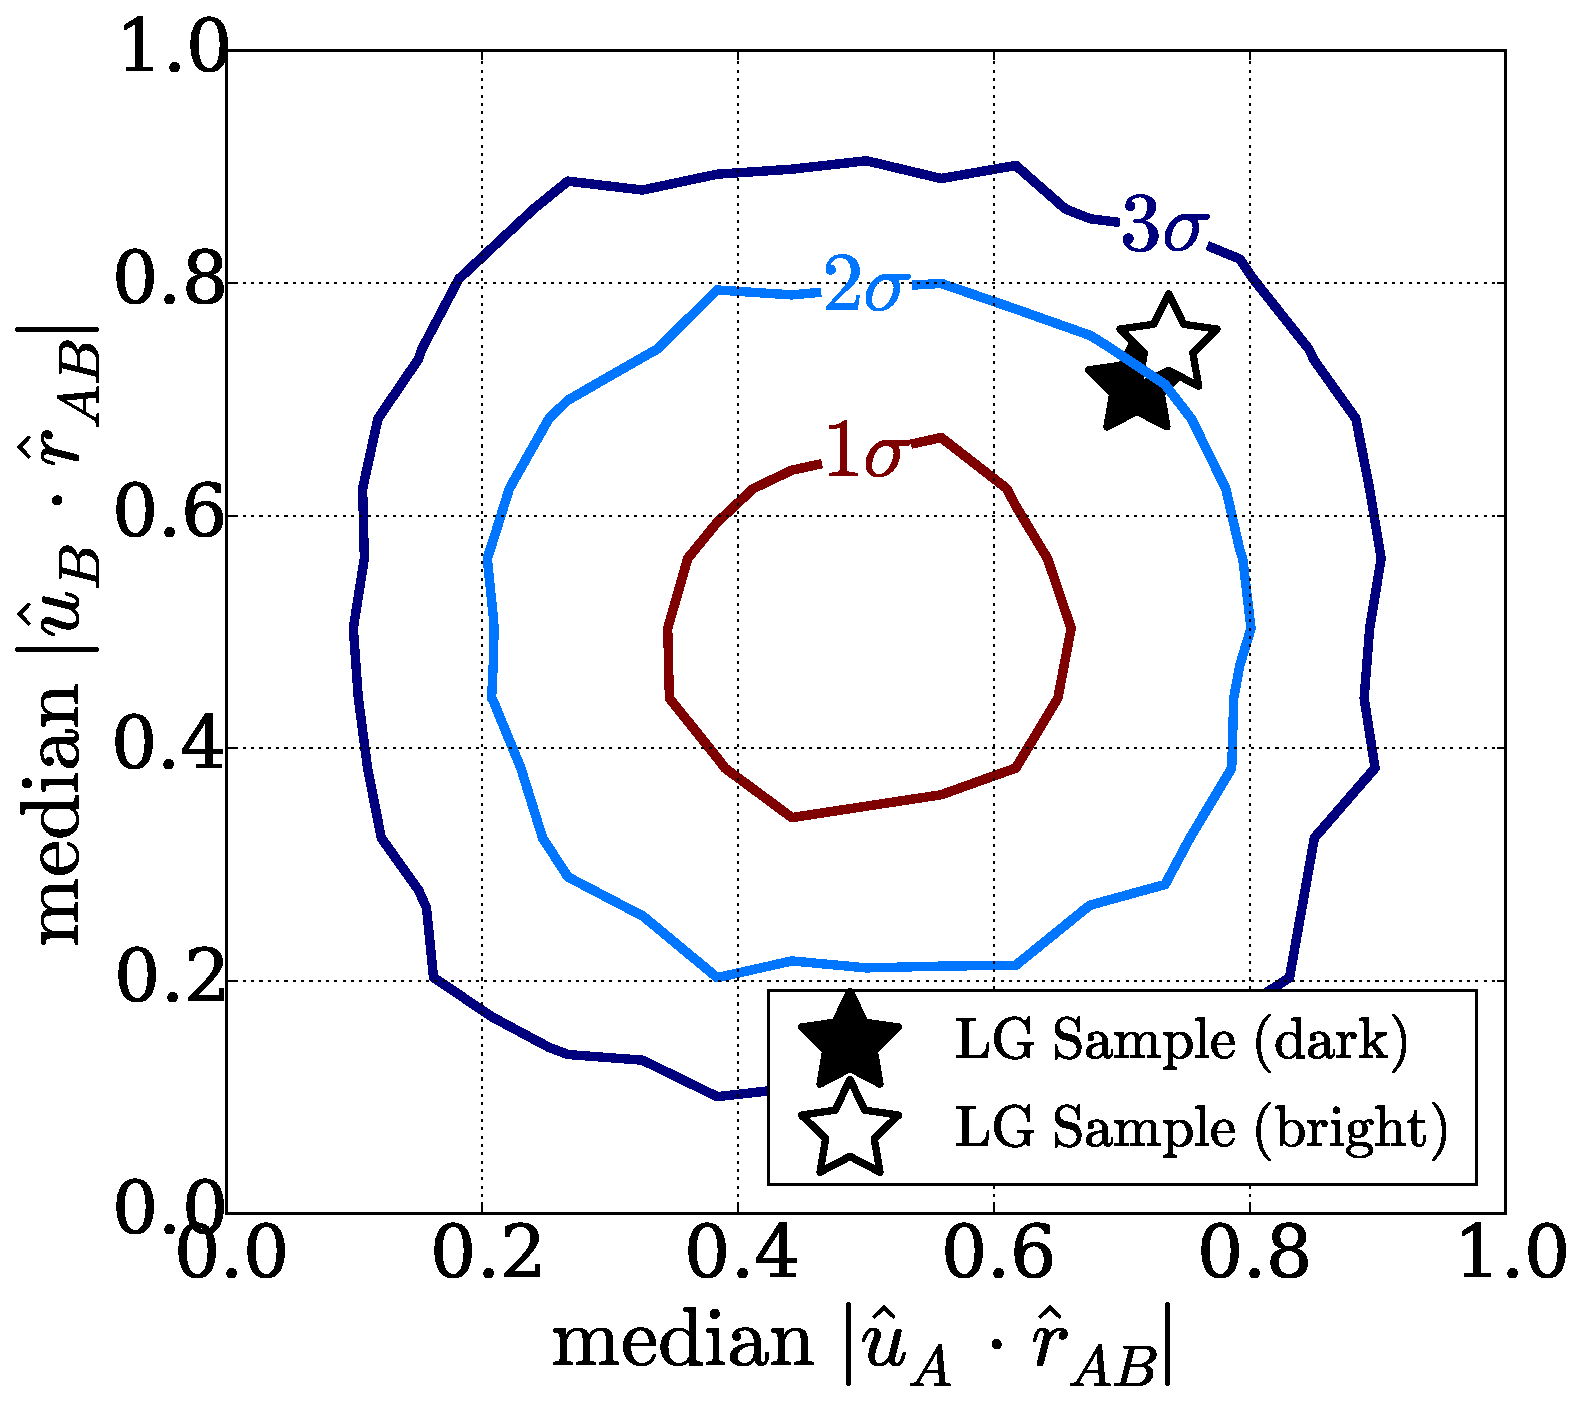
\includegraphics[width=0.48\hsize]{significance_lg_bright.pdf}
\caption{Significance of alignments.}
\label{fig:significance}
\end{figure*}

\begin{figure}
\centering
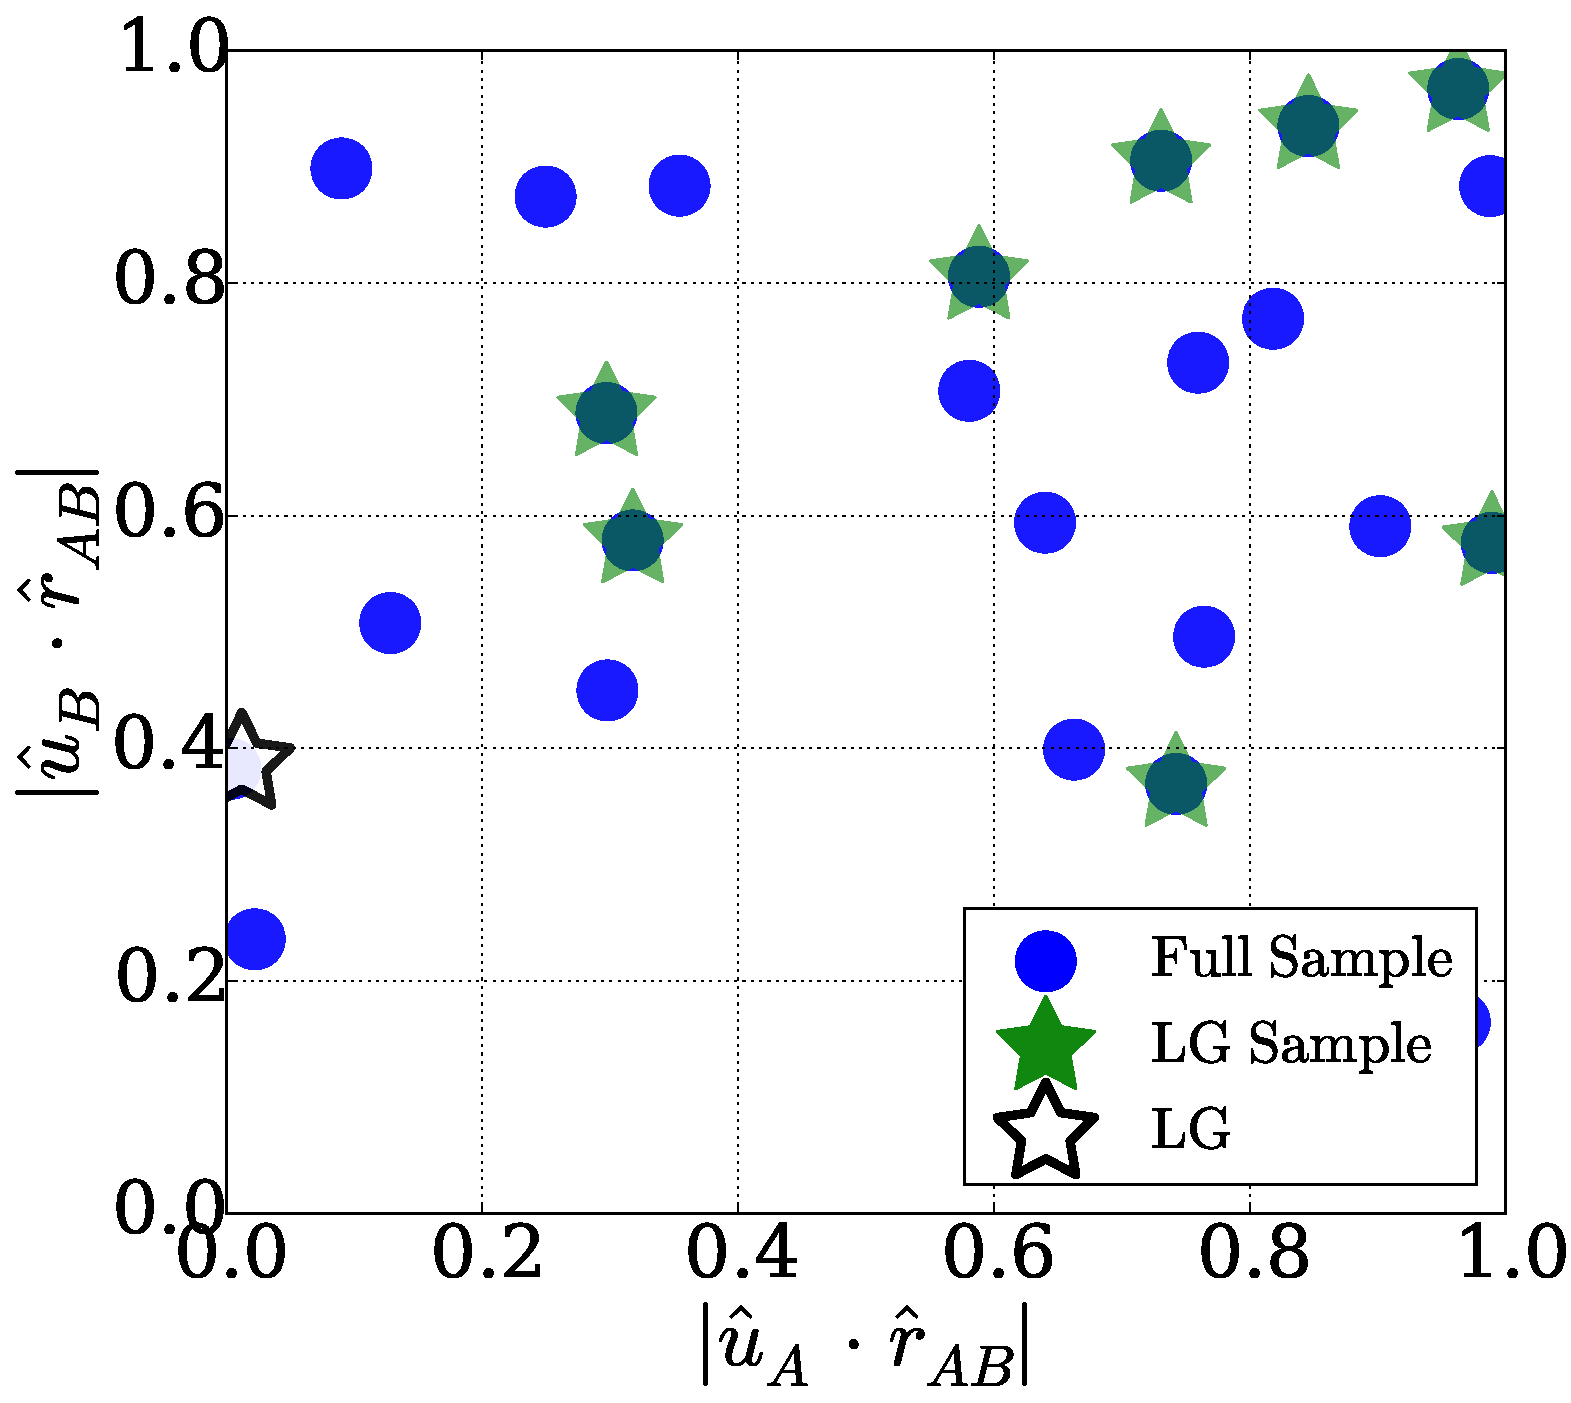
\includegraphics[width=\hsize]{r_u_alignment.pdf}\\
\caption{Alignment of the mayor axis with the vector connecting the
  two halos.}
\label{fig:lg_alignment}
\end{figure}

\begin{figure}
\centering
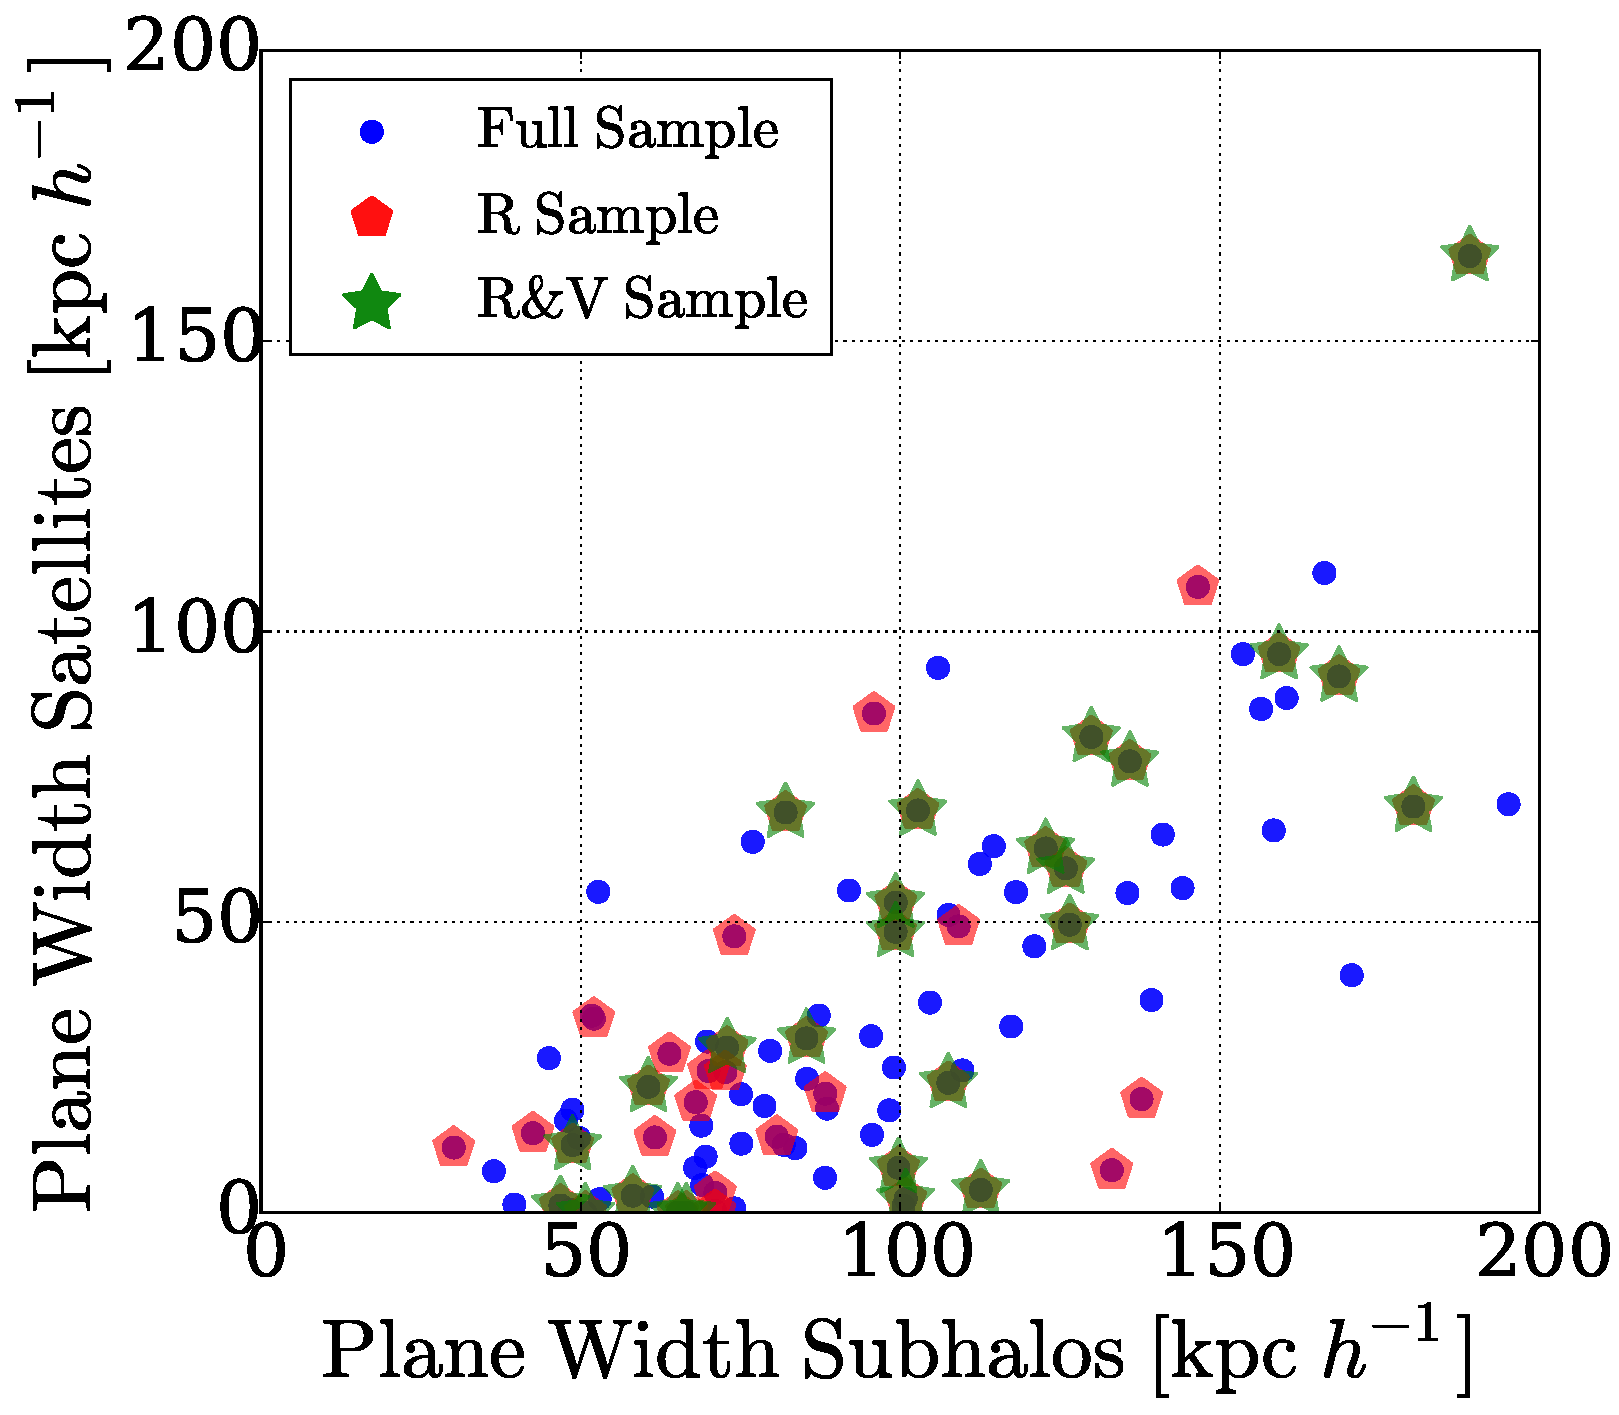
\includegraphics[width=\hsize]{plane_width.pdf}\\
\caption{Plane width for the best planes in the luminious and dark cases.}
\label{fig:plane_width}
\end{figure}

\begin{figure}
\centering
\includegraphics[width=\hsize]{plane_width_n_dark.pdf}\\
\caption{Plane width as a function of objects used to find the plane.}
\label{fig:plane_width_nobjects}
\end{figure}

\section{Results}
\label{Results}

\section{Method}
\label{Method}



%\begin{figure}
%\centering
%\includegraphics[width=\hsize]{Halo_pos_LRomulusRemus.pdf}\\
%\end{figure}

\section{Discussion} 
\section{Acknowledgements}
Gracias.

%\begin{wraptable}{l}{2\linewidth}
%\centering
%\begin{tabular}{|l|l|l|l|l|l|}
%\hline
%Bahl 2013       & MilleniumII & resolution & number of host halos& gas no        & planes yes? \\\hline
%Ibata 2014      & MilleniumII & resolution & number of host halos& gas no        & planes no? \\\hline
%Pawlowski 2015  & MilleniumII & resolution & number of host halos& gas no        & planes no? \\\hline
%Gillet 2015     & CLUES       & resolution & number of host halos& gas yes and no& planes yes \\\hline
%Cautun 201XXX   & ?           & resolution & number of host halos& gas ??????    & planes yes \\\hline
%Buck            & their own   & resolution & number of host halos& gas no?       & planes yes \\\hline
%Sawala          & Apostole?   & resolution & number of host halos& gas yes?      & planes yes \\\hline
%Gonzalez        & their own?  & resolution & number of host halos& gas yes/no    & planes he does not care \\\hline
%\end{tabular}
%\end{wraptable}

Simulation papers:
\begin{itemize}
\item{Bahl and Baumgardt 2013 "A comparison of the distribution (...)":\\
MilleniumII and a semi-analytic model\\
Baryonic mass cut: 2.8$\times 10^4 M\odot$\\
PAndAS like field\\
With orphan galaxies: planes are common (40$\%$) but overall distribution is different from that of M31 (more radially concentrated).\\
Excluding \emph{some} orphan galaxies: overall distribution closer to M31's and finds planes.\\
Conclusion: M31 like planes are not uncommon in MilleniumII simulations. Co-rotating structures are not stable structures. Plane of M31 could be a statistical fluctuation in an otherwise more spherical distribution.\\
Simulation: Millenium II ()\\
Gas: NO\\
Resolution: sub-halos 2$\times 10^8 M\odot$ (orphan galaxies have less than 20 particles and could be tidally disrupted)\\
Number of host halos: 1511 with orphan galaxies, 112 excluding orphan galaxies (mass between 1.1$\times 10^{12} M\odot$ and 1.7$\times 10^{12} M\odot$), younger that 10 Gyr and satelites smaller than 7$\times 10^{10} M\odot$\\
Planes: yes (40$\%$ with orphan galaxies 2$\%$ without)\\
co-rotation: yes (in 2$\%$ of the halos ???)\\
Stable: No\\
Note: PAndAS data has satellites with baryonic masses down to 2.9$\times 10^{4} M\odot$ and they take that as a lower limit for their data.\\
}
\item{Ibata et al 2014 "A thousand shadows (...)":\\
MilleniumII and a semi-analytic model (Guo)\\
%Baryonic mass cut: 2.8$\times 10^4 M\odot$\\
Same analysis as in PAndAS data\\
%With orphan galaxies: planes are common (40$\%$) but overall distribution is different from that of M31 (more radially concentrated).\\
%Excluding \emph{some} orphan galaxies: overall distribution closer to M31's and finds planes.\\
Conclusion: M31 like planes are NOT common in MilleniumII simulations.\\
Simulation: Millenium II ()\\
Gas: NO\\
Resolution: sub-halos 2$\times 10^8 M\odot$ (orphan galaxies have less than 20 particles and could be tidally disrupted)\\
Number of host halos: 679 (I assume with orphan galaxies) (mass between 1.1$\times 10^{12} M\odot$ and 1.7$\times 10^{12} M\odot$, younger that 10 Gyr and satellites smaller than 7$\times 10^{10} M\odot$ they also use LG upper mass limit, and an isolation criteria).\\
Planes: no (with orphan galaxies only 0.04$\%$ of the system fulfill the thinness, extension and co-rotation criteria, and NONE does if orphans are not included. If co-rotation is not included then $2\%$ fulfill the thinness and extension criteria)\\
co-rotation: only 0.04$\%$ with orphans and NONE without orphans\\
Note: they use the 679 host halos and study them from different viewing angles\\
}
\item{Pawlowski et al 2014 "Co-orbitingsatellite galaxy structures are still in conflict with (...)":\\
MilleniumII and a semi-analytic model (Guo)\\
%Baryonic mass cut: 2.8$\times 10^4 M\odot$\\
Same analysis as in PAndAS data\\
Same analysis as in Wang et al. 2013\\
%With orphan galaxies: planes are common (40$\%$) but overall distribution is different from that of M31 (more radially concentrated).\\
%Excluding \emph{some} orphan galaxies: overall distribution closer to M31's and finds planes.\\
Conclusion: M31 and MW like planes are NOT common in MilleniumII simulations.\\
Simulation: Millenium II ()\\
Gas: NO\\
Resolution: sub-halos 2$\times 10^8 M\odot$ (orphan galaxies have less than 20 particles and could be tidally disrupted)\\
Number of host halos:  1825 (mass between 1.1$\times 10^{12} M\odot$ and 1.7$\times 10^{12} M\odot$, younger that 10 Gyr and satellites smaller than 7$\times 10^{10} M\odot$ they also use LG upper mass limit, and an isolation criteria).\\
Planes: no (M31: 0.09$\%$ fulfill the thinness, extension and co-rotation criteria. MW: 0.2$\%$)\\
Note: they use the host halos and study them from different viewing angles so they end up with 15000 samples. They always consider orphan galaxies for comparison purposes. For one test they randomize the sample and find M31 like planes in only 0.002 per cent of the cases and MW like planes in 0.06$\%$ of the cases.\\
MIRAR Wang et al. 2013 que busca MWlike planes en MilleniumII y encuentra que $13\%$ de los halos tienen planos
}
\item{Cautun et al. 2015 "Planes of satellite galaxies: when exceptions are the rule":\\
MilleniumII and a semi-analytic model (Guo 2013)\\
CoCo and a semi-analytic model (Guo 2015)\\
%Baryonic mass cut: 2.8$\times 10^4 M\odot$\\
Conclusion: planar structures are very common in $\Lambda$CDM (10$\%$)\\
Simulation 1: Millenium IIi rescaled to WMAP\\
Simulation 2: CoCo (Higher resolution than MilleniumII)\\
Gas: NO\\
Resolution 1: sub-halos 2$\times 10^8 M\odot$ (orphan galaxies have less than 20 particles and could be tidally disrupted)\\
Number of host halos:  2849 (MilleniumII) and 63 8COCO halos) (selection criteria: "we adopted a broader mass range to account for the large uncertainty in the mass measurements and also for possible systematic effects").\\
Resolution 2: sub-halos $\approx$ 2$\times 10^6 M\odot$ (75 times higher mass resolution
and four times better spatial resolution)\\
Planes: yes (10$\%$)\\
Note: They found a great variety of plane and the M31 plane lies in general within the scatter of the simulated planes however it seem to have an "unusually large radial extent".\\
Note 2: they find that each halos has a different planar configuration showing that the low incidence of the M31 plane is not in contradiction with simulations. This contradicts the Pawlowski et al. 2014 conclusions}
\end{itemize}




\bibliographystyle{apj}
\bibliography{Dwarfs}

\end{document}

